\chapter{Results} \label{ch:resultados}

This section provides the main results of the investigation. The main functions used to obtain these results are shown in the Appendix \ref{ch:Anexo}. 
The results are divided into three sections:
\begin{enumerate}
    \item First, the results reproduced from the original paper \cite{notarmuzi2021percolation} are presented.
    \item Secondly, we will present the same analysis for the case of a Hawkes process with $n=2$.
    \item Finally, we will study the behaviour of two Hawkes processes couples, one representing an excitatory neuron and the other an inhibitory neuron.
\end{enumerate}

\section{Results from the original paper}

The structure for the three sections will be the same. First, we will obtain the phase diagram for the percolation strength $P_{\infty}$ versus our control parameter, the resolution parameter 
$\Delta$, obtaining the critical(s) point(s) $\Delta^*_{i}$. Having these in knowledge, the avalanche statistics for the size and duration will be studied for different regions 
of the phase diagram.  

As previosly stated, the first result is the percolation phase diagram, shown in Figure \ref{f:phase_diagram_article}. 
It displays the percolation strength $P_{\infty}$, which is the number of events in the largest cluster divided by the total number of events of the time series
versus the resolution parameter $\Delta$. We will generate several time series, compute the percolation strength for each one and take the average value.

\begin{figure}[H]
    \centering
    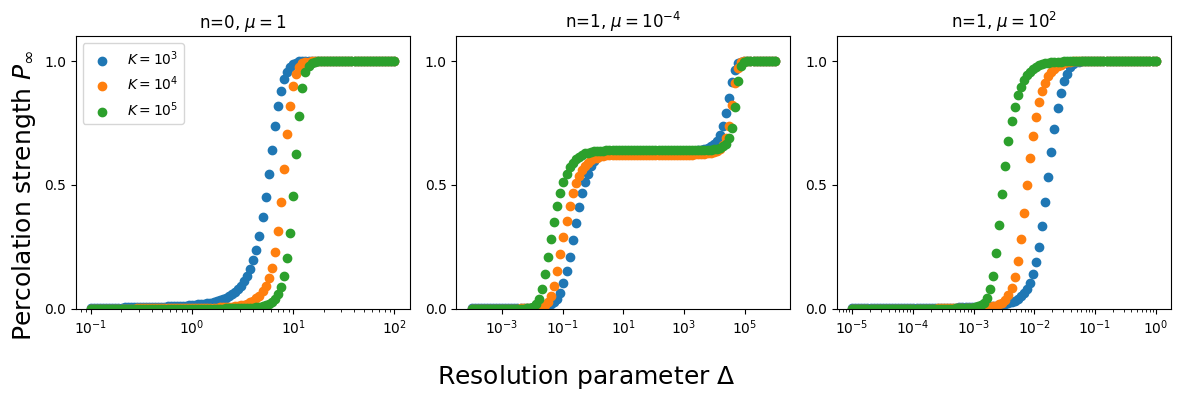
\includegraphics[width=0.95\textwidth]{phase_article_R=1000.png}
    \caption{Percolation phase diagrams for different event number $K$ taking average values of $R=1000$ realizations.}
    \label{f:phase_diagram_article}
\end{figure}

The first plot configuration is a homogeneous Poisson process with rate $\mu=1$ which we have overviewed in Section \ref{subsec:Poisson_processes} and has a pseudocritical threshold at 
$\Delta^*(K)=\frac{\ln(K)}{\mu}$ as we have demonstrated in Section \ref{sec:physics_cooking}. Due to the fact of finite size of the time series, the transition is discontinuous at 
the threshold, as expected for 1D percolation \cite{stauffer2018introduction}.

Now, we contemplate Hawkes processes, for the first case $\left( \mu=10^{-4} \right)$, we can observe a double discontinuous transition. The first one at $\Delta_1^*$ and the second one at
$\Delta_2^*$. As we are going to see with the avalanche statistics, the first transition is associated with the universality class of 1D percolation whose exponents are $\alpha=\tau=2$. 
On the other hand, the second transition is associated with the universality class of mean-field branching process whose exponents are $\alpha=3/2$ and $\tau=2$. This double transition 
is also compatible with the fact mentioned in Figure \ref{f: Delta percolación}. We can also observe that the plateau between the two transitions is wider as the $K$ increases as expected.
For the second case $\left( \mu=10^2 \right)$, similarly to the first one, we have a single discontinuous transition at $\Delta_1^*$ associated with the universality class of 1D percolation
as well, this phenomenon is also compatible with the one shown in Figure \ref{f: Delta percolación 2}.

Another interesting analysis to characterize the phases is studying the susceptibility $\chi$. In this case, it is defined by Eq \ref{eq:susceptibilidad}.

\begin{equation}
    \begin{split}
        \chi =& \dfrac{ \langle S_M^2 \rangle - \langle S_M \rangle^2 }{\langle S_M \rangle}\\
             =& K\cdot \dfrac{\langle P_{\infty}^2 \rangle - \langle P_{\infty} \rangle^2}{\langle P_{\infty} \rangle}\\
             =& K\cdot \dfrac{\sigma^2\left( P_\infty \right)}{\langle P_{\infty} \rangle}
    \end{split}
    \label{eq:susceptibilidad}
\end{equation}

The susceptibility (normalized to the number of events) is shown in Figure \ref{f:susceptibilidad_article}. For the Poisson process, we see that the susceptibility has a peak at the
the threshold $\Delta^*(K)$, then it vanishes as expected. For the Hawkes case with $\mu=10^{-4}$, we observe that $\chi$ has a peak at the critical point $\Delta_1^*$, then 
we have a critical behaviour where the susceptibility is not zero at the plateau $[\Delta_1^*,\Delta_2^*]$ and finally, it vanishes at the second critical point $\Delta_2^*$. Finally, 
for the Hawkes case with $\mu=10^2$ and likewise the Poisson process, the susceptibility has a divergence at the critical point $\Delta_1^*$ and then it vanishes. 

\begin{figure}[H]
    \centering
    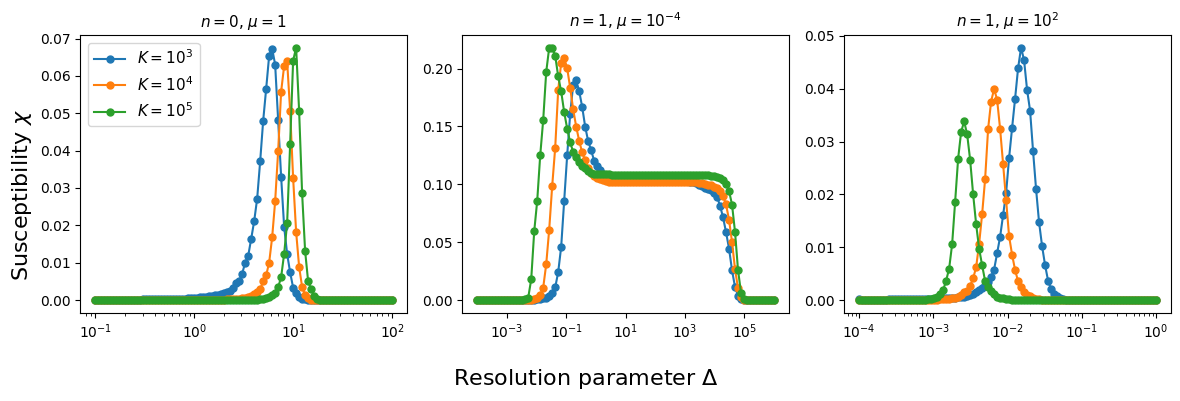
\includegraphics[width=0.95\textwidth]{susceptibilidad n=1.png}
    \caption{Susceptibility $\chi$ normalized to the number of evetns $K$, for different event number $K$ and taking average values for $R=1000$ realizations.}
    \label{f:susceptibilidad_article}   
\end{figure}

Once we have the phase diagram, we can study avalanche statistics, but first, we need to obtain the thresholds $\Delta_1^*$ and $\Delta_2^*$ from the phase diagram. 
The article \cite{notarmuzi2021percolation} provides the following formulas to compute these thresholds for the Hawkes process with $\mu=10^{-4}$ and:

\begin{align}
    \Delta_1^* &\simeq \dfrac{\ln(K)}{\langle \lambda \rangle}= \dfrac{\ln(K)}{\mu+\sqrt{2\mu K}} \label{eq:Ecuación delta1 *} \\
    \Delta_2^* &= \dfrac{\ln(K)}{\mu}\label{eq:Ecuación delta2 *}
\end{align}

and for $\mu=10^2$:

\begin{equation}
    \Delta_1^* = \dfrac{\ln(K)}{\mu}
\end{equation}

Bearing this in mind and the definitions of the size and duration of avalanches established in the previous chapter, we can study the avalanches for the different regions
of the phase diagram. We just are going to show the results for $\mu=10^{-4}$ and for $\mu=10^2$ in Figure \ref{f:avalanches_article}. The Poisson process behaviour can be found in 
\cite{stauffer2018introduction, stauffer1978critical}. 


\begin{wrapfigure}{l}{0.65\textwidth}
    \begin{center}
      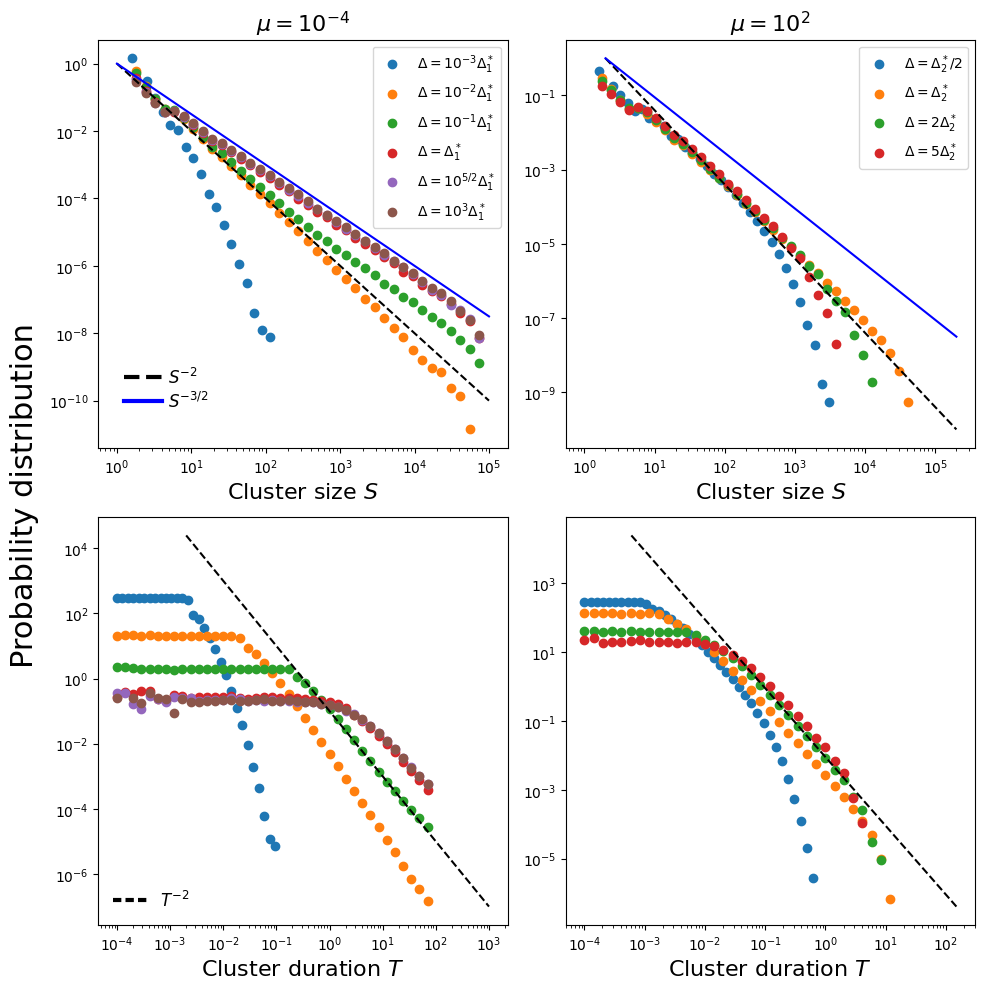
\includegraphics[width=0.6\textwidth]{stats article.png}
    \end{center}
    \caption{Avalanche analysis for Hawkes process with $n=1$, $K=10^5$ events averaged over $R=1000$ realizations.}
    \label{f:avalanches_article}
\end{wrapfigure}

As a consequence of the huge simulation time of time series of $K=10^8$ events, we have only studied the avalanches for $K=10^5$, moreover, we have taken other criterion to obtain the 
histograms. Instead of considering $C=10^7$ clusters, we have obtained the histograms of $R=1000$ time series. This leads to a different amount of clusters for each value of $\Delta$, 
nevertheless, we have obtained equivalent and reliable results.  

For $\mu=10^{-4}$, the probability distribution of the cluster size and duration shows three different behaviours. For $\Delta\ll\Delta_1^*$, the behaviour is subcritical, leading to
to a exponential decay for the size and duration. While we increase $\Delta$, we reach the critical point where the exponents are $\alpha=\tau=2$ compatible with the universality class
of 1D percolation. After that, we reach the plateau $[\Delta_1^*,\Delta_2^*]$ where we have a crossover to the universality class of mean-field branching process and 1D percolation. 
Finally, for $\Delta\to\Delta_2^*$, we obtain the universality class of mean-field branching process exponents $\alpha=3/2$ and $\tau=2$. 
For $\mu=10^2$, the plots show a power-law distribution for both cluster size and duration with exponents $\alpha=\tau=2$ corresponding to the universality class of 1D percolation as we have
mentioned before.  

Note that we have reproduced the same behaviour, but for other values of $\Delta$, specifically, for two order of magnitude less than article value. This is due 
to the fact that Eq. \ref{eq:Ecuación delta1 *} needs the assumption of large time series, condition which is not fulfilled in our case. We can illustrate this difference 
for example in the susceptibility diagram, where the peak should be at $\Delta_1^*$, but in our case, it is at $\Delta_1^*/100$ as shown in Figure \ref{f:different delta1estrella}. 

\begin{figure}[H]
\centering
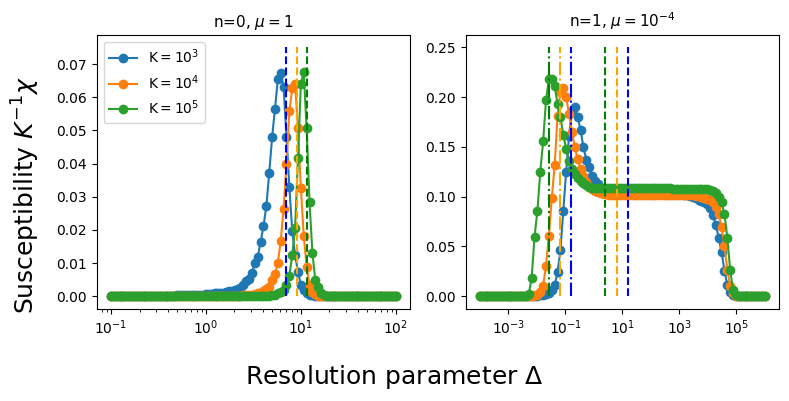
\includegraphics[width = 0.7\textwidth]{different delta1estrella.png}
\caption{At the left, the vertical dashed lines represent the critical points $\Delta^*(K)$ for the Poisson process. At the right, the vertical dashed lines represent 
the critical points $\Delta_1^*(K)$ given by Eq. \ref{eq:Ecuación delta1 *} and the dotted dashed lines the $\Delta_1^*/100$.} 
\label{f:different delta1estrella}
\end{figure}




\section{Results for n=2}

In the article, the authors have studied a process which is critical itself because the parameter $n$ is fixed to $n=1$. We have studied the case $n=2$ to see if the process is still critical. 
In the Figure \ref{f:n=1 vs n=2} two time series for $n=1$ and $n=2$ are shown. 

\begin{figure}[H]
    \centering
    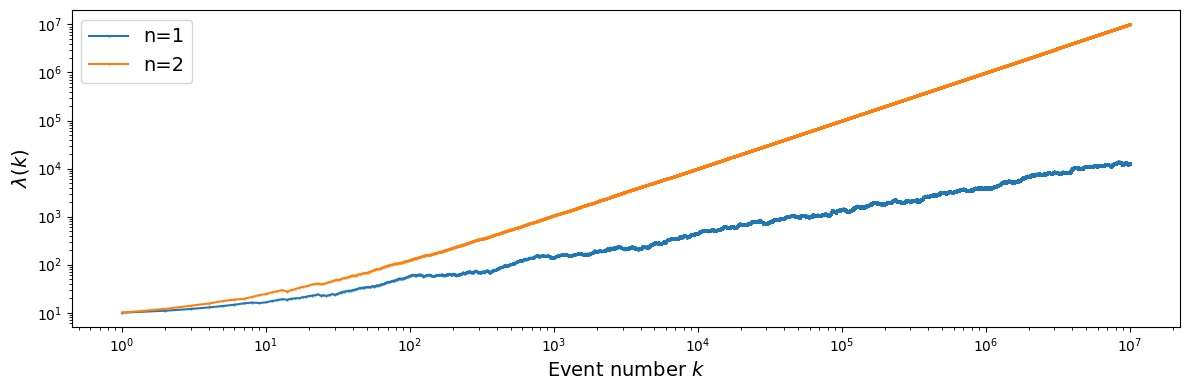
\includegraphics[width=0.65\textwidth]{n=1 vs n=2.png}
    \caption{Time series for $n=1$ and $n=2$.}
    \label{f:n=1 vs n=2}
\end{figure}

Similarly to the previous section, first we obtain the phase diagram in order to observe the transitions. In this case, Eqs. \ref{eq:Ecuación delta1 *},\ref{eq:Ecuación delta2 *} are not valid.
Therefore, we will obtain this parameter graphically from the phase diagrams shown in Figure \ref{f:phase_diagram_n=2}.
\begin{figure}[H]
    \centering
    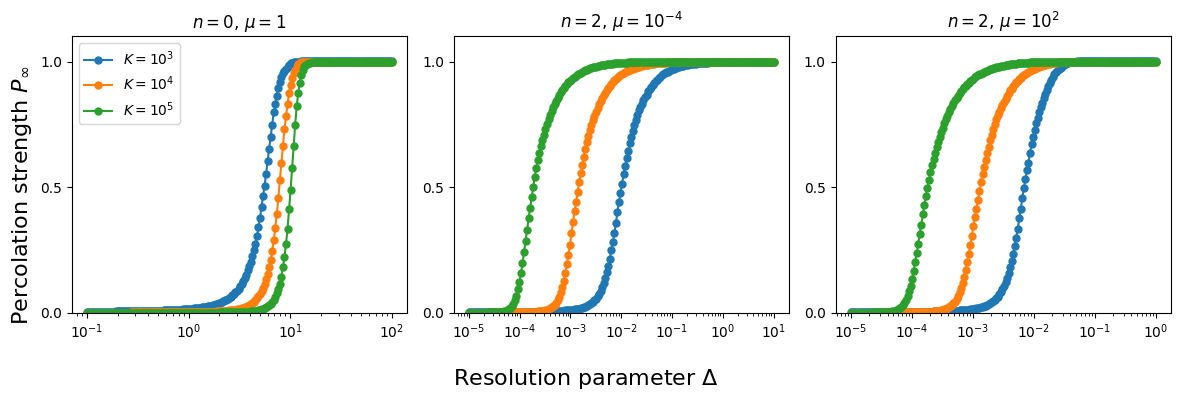
\includegraphics[width=0.95\textwidth]{phase_R=1000_n=2.png}
    \caption{Percolation phase diagrams for a Hawkes process with $n=2$.}
    \label{f:phase_diagram_n=2}
\end{figure}

As we can see, now we have a single transition for $\mu=10^{-4}$ and $\mu=10^2$ corresponding to 1D percolation, consequently, the exponents for the size and duration 
should be $\alpha=\tau=2$. In a similar way, we have studied the avalanches for $K=10^5$ events and $R=1000$ realizations to obtain the average values. The statistics of the avalanches 
are shown in Figure \ref{f:avalanches_n=2}.


\begin{wrapfigure}{l}{0.75\textwidth}
    \begin{center}
      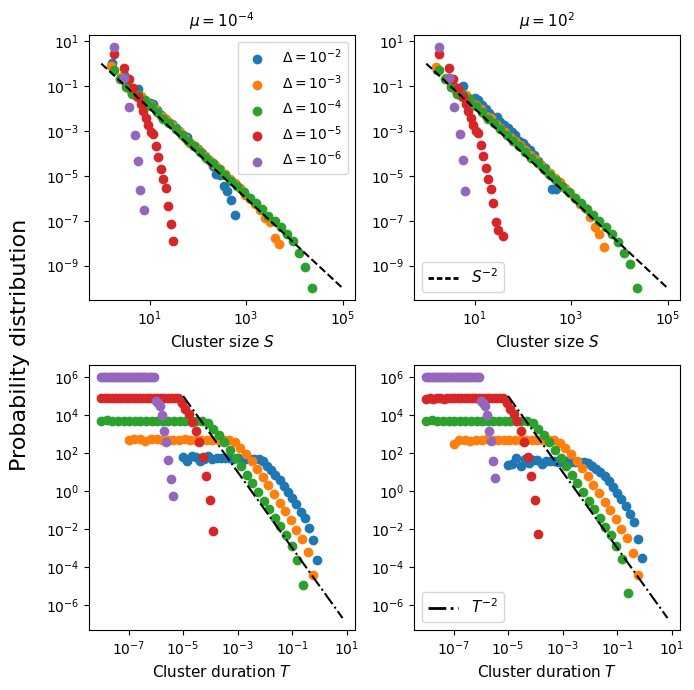
\includegraphics[width=0.675\textwidth]{cutoff_data_dots_n=2.png}
    \end{center}
    \caption{Avalanche statistics for a self-exciting Hawkes process with $n=2$ for $K=10^5$ events averaged over $R=1000$ realizations.}
    \label{f:avalanches_n=2}
\end{wrapfigure}
\clearpage
\section{Inhibitory and excitatory neurons coupled}
